%****************************************************************
% Chapter X
%****************************************************************
\label{ChapterX}
\chapter{Chapter X}

%****************************************************************
\section{Sphere}

Introduce UV sphere and Icosphere generation.

\subsection{UV Sphere}

The UV sphere, somewhat like latitude and longitude lines of the earth, uses rings and segments. Near the poles (both on the Z-axis with the default orientation) the vertical segments converge on the poles. UV spheres are best used in situations where you require a very smooth, symmetrical surface.

\begin{figure}[H]
\centering
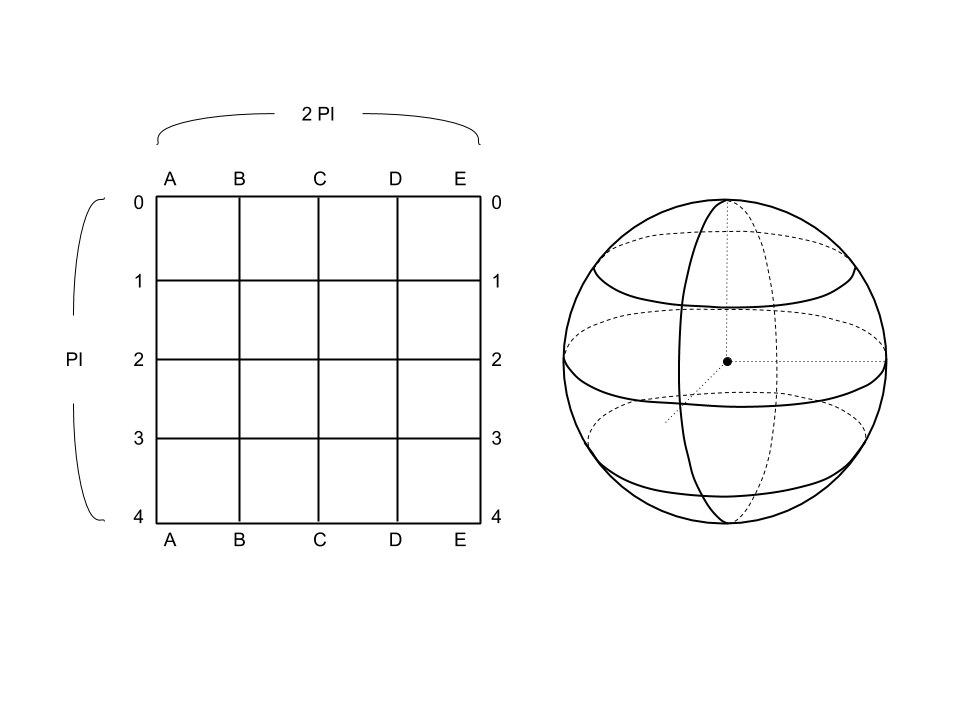
\includegraphics[width=\linewidth]{Figures/uv-sphere-mapping.png}
\decoRule
\caption[uv-sphere-mapping]{UV sphere mapping}\label{fig:uv-sphere-mapping}
\end{figure}

As we can see the mapping from \ref{flg:uv-sphere-mapping}. Vertex $A0,\;A1,\;A2,\;A3,\;A4$ and $E0,\;E1,\;E2,\;E3,\;E4$ are duplicated, and $A0,\;B0,\;C0,\;D0,\;E0$ converge together as well as $A4,\;B4,\;C4,\;D4,\;E4$. So we can simply define it as a UV sphere has 5 rings and 4 segments. Also be noticed that each ring spans $2\,\pi$ radians, but each segment spans $\pi$ radians in the sphere mapping.

The total vertex number is:

\begin{equation}\label{equ:uv-sphere-vertices}
Vertices = Rings \times Segments
\end{equation}

\begin{figure}[H]
\centering
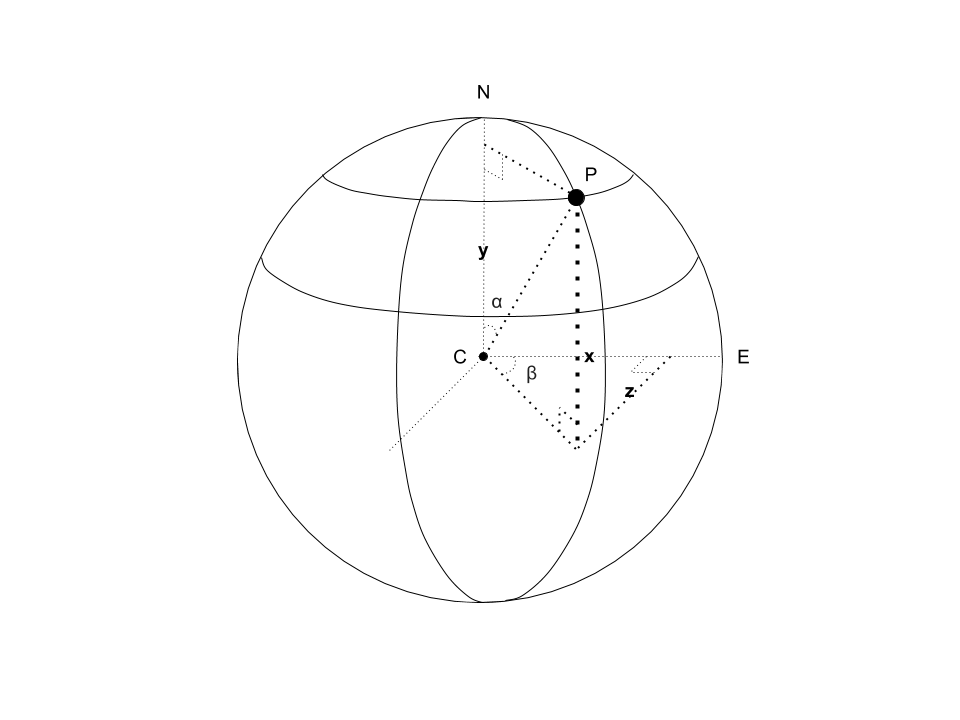
\includegraphics[width=\linewidth]{Figures/uv-sphere-vertex.png}
\decoRule
\caption[uv-sphere-vertex]{UV sphere vertex}\label{fig:uv-sphere-vertex}
\end{figure}

For each vertex $P$ on sphere from ring $r$ and segment $s$, we have:

\[
\begin{array}{lr}
v = r \times  \frac{1}{rings - 1} \\
u = s \times  \frac{1}{segments - 1} \\
\measuredangle \alpha = v \times \pi \\
\measuredangle \beta = u \times 2\,\pi \\
\end{array}
\]

$\therefore$ P (x,\;y,\;z)
\[
\begin{array}{lr}
x = (\sin(\alpha) \times radius) \times \cos(\beta) \\
y = \cos(\alpha) \times radius \\
z =  (\sin(\alpha) \times radius) \times \sin(\beta)
\end{array}
\]

When raduis equals 1:

\[
\begin{array}{lr}
x = \sin(\alpha) \times \cos(\beta) \\
y = \cos(\alpha) \\
z =  \sin(\alpha) \times \sin(\beta)
\end{array}
\]


\subsection{Icosphere}

Figure \ref{fig:icosahedron-rectangles} shows that the initial vertices of an icosahedron are the corners of three orthogonal rectangles:

\begin{figure}[H]
\centering
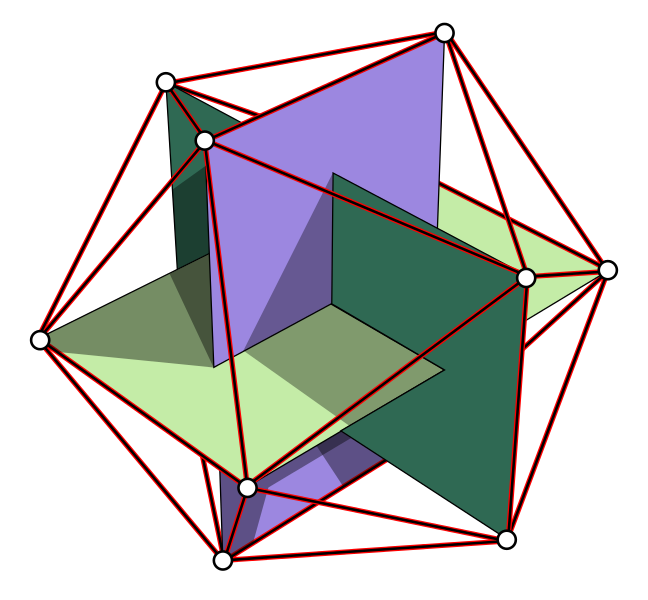
\includegraphics[width=\linewidth]{Figures/icosahedron-rectangles.png}
\decoRule
\caption[icosahedron-rectangles]{Icosahedron rectangles \parencite{wiki.icosahedron-rectangles.2006}}\label{fig:icosahedron-rectangles}
\end{figure}

Rounding icosphere by subdividing a face to an arbitrary level of resolution. One face can be subdivided into four by connecting each edge's midpoint.

\begin{figure}[H]
\centering
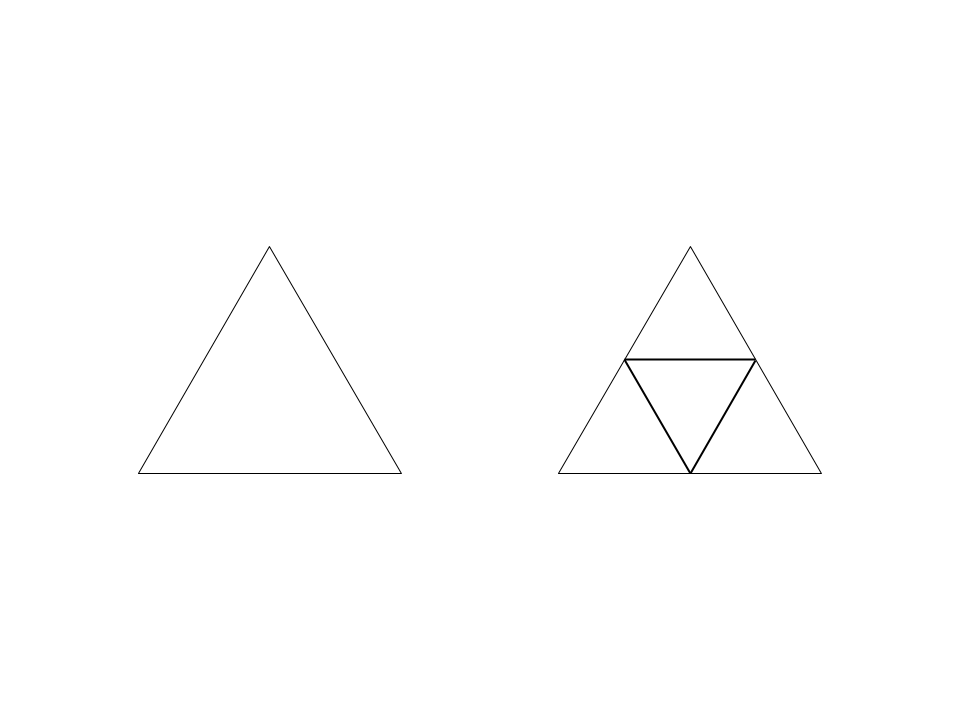
\includegraphics[width=\linewidth]{Figures/icosphere-subdivide.png}
\decoRule
\caption[icosphere-subdivide]{Icosphere subdivide}
\end{figure}

Push edge's midpoints to surface of the sphere.

\begin{figure}[H]
\centering
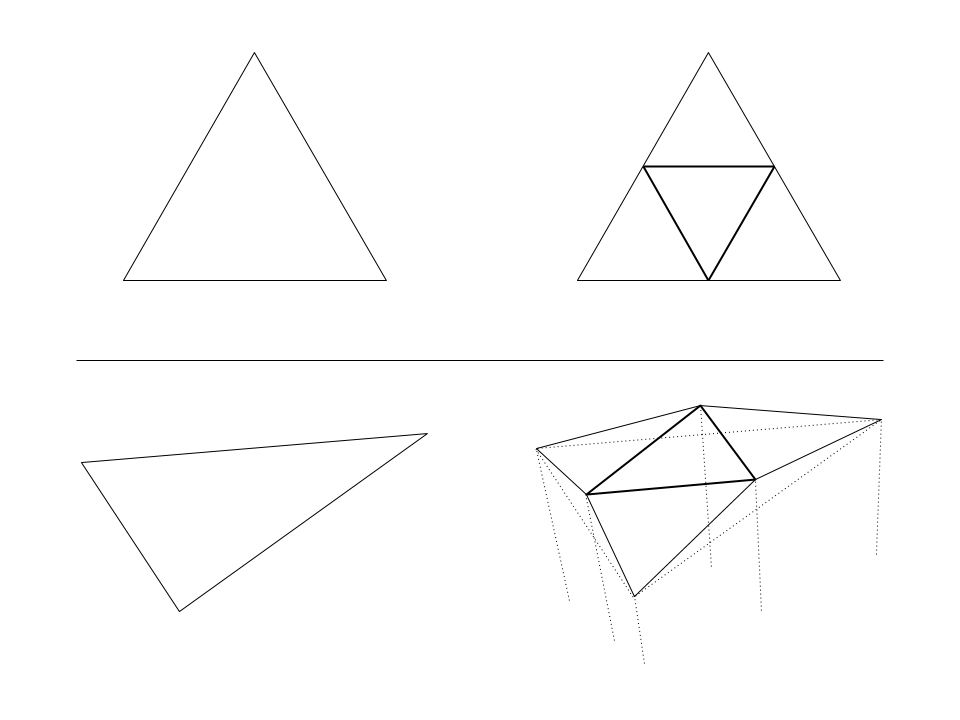
\includegraphics[width=\linewidth]{Figures/icosphere-refinement.png}
\decoRule
\caption[icosphere-refinement]{Icosphere refinement}
\end{figure}





%****************************************************************
\section{Camera Movement}

In general, there are two sensors can be useful to manager camera movement: ACCELEROMETER (API level 3), LINEAR\_ACCELERATION (API level 9) and STEP\_DETECTOR (API level 19). 

LINEAR\_ACCELERATION is same as ACCELERATION which measures the acceleration force in meter per second repeatedly, except linear acceleration sensor is a synthetic sensor with gravity filtered out. 

\[
\begin{array}{lr}
Linear Acceleration = Accelerometer Data - Gravity \\
v = \int a\,dt \\
x = \int v\,dt
\end{array}
\]

First of all, we take the acclerometer data and remove gravity that is called gravity compensation, whatever is left is linear movement. Then we have to integrate it one to get velocity, integrated again to get position, which is called double integral. Now if the first integral creates drift, double integrals are really nasty that they create horrible drift. Because of these noise, using acceleration data it isn't so accurate, it is really hard to do any kind of linear movement \parencite{GoogleTechTalks.sensor-fusion.2010}.

On the other hand, use step counter from STEP\_DETECTOR, and pedometer algorithm for pedestrian navigation, that in fact works very well for this project.

\[
\begin{array}{lr}
p_1 = p_0 + v_0 \times dt \\
v_1 = v_0 + a \times dt
\end{array}
\]

The accuracy of this depends on how precision we can get for changing velocity. Considering that velocity is made of 3-axis directions, the current heading direction is required for a correct velocity calculation. Since the frame life cycle is implemented based on \parencite{Google.VR-SDK.2016}, which provide the heading direction in each frame callback. So I collect everything I need from the last frame to new frame, and update both velocity and position for each new frame.

For updating process, first of all, 

First of all, damping is required. I reduce velocity by a percentage. It is simply for avoiding that camear taking too long to stop. Damping by percentage can stable and stop the camera in a certain of time that won't be affected by the current camera speed. 


Secondly, a constant value in head forwarding direction is been used as a pulse for each step. Because a step is happening instantaneously which implies $a\,dt$ made by each step is actually can be replace by a constant value.

\begin{figure}[H]\label{fig:camera-movement}
\centering
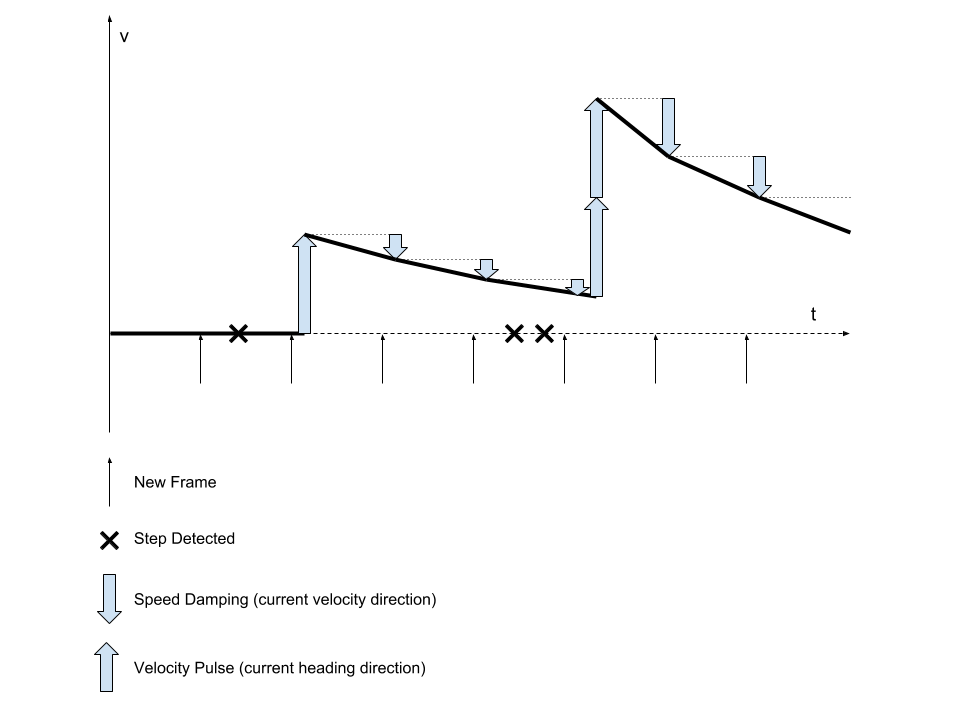
\includegraphics[width=\linewidth]{Figures/camera-movement.png}
\decoRule
\caption[camera-movement]{Camera movement}
\end{figure}

For each new frame:

\[
\begin{array}{lr}
\begin{aligned}
\overrightarrow{V_0} &= \overrightarrow{V_0} \cdot Damping \\
\overrightarrow{P_1} &= \overrightarrow{P_0} + \overrightarrow{V_0} \cdot dt \\
\overrightarrow{V_1} &= \overrightarrow{V_0} + \overrightarrow{Forwarding} \cdot Pulse \cdot Steps \\
Damping &\in [0,\enspace1] \\
Pulse &\in [0,\enspace \infty)
\end{aligned}
\end{array}
\]

%****************************************************************
\section{Ray Intersection}

Detect collisions between ray and models is the key to allow user selecting objects in the VR would, which is one of the importent experience for user interaction.

A ray can be describe in a equation with known ray start position \emph{$\overrightarrow{R_0}$} and ray direction \emph{$\overrightarrow{R_d}$}.

\begin{equation}\label{equ:ray-t}
\overrightarrow{R(t)} = \overrightarrow{R_0} + \overrightarrow{R_d} \cdot t
\end{equation}

%****************************************************************
\subsection{Ray-Sphere}

\begin{figure}[H]\label{fig:ray-sphere}
\centering
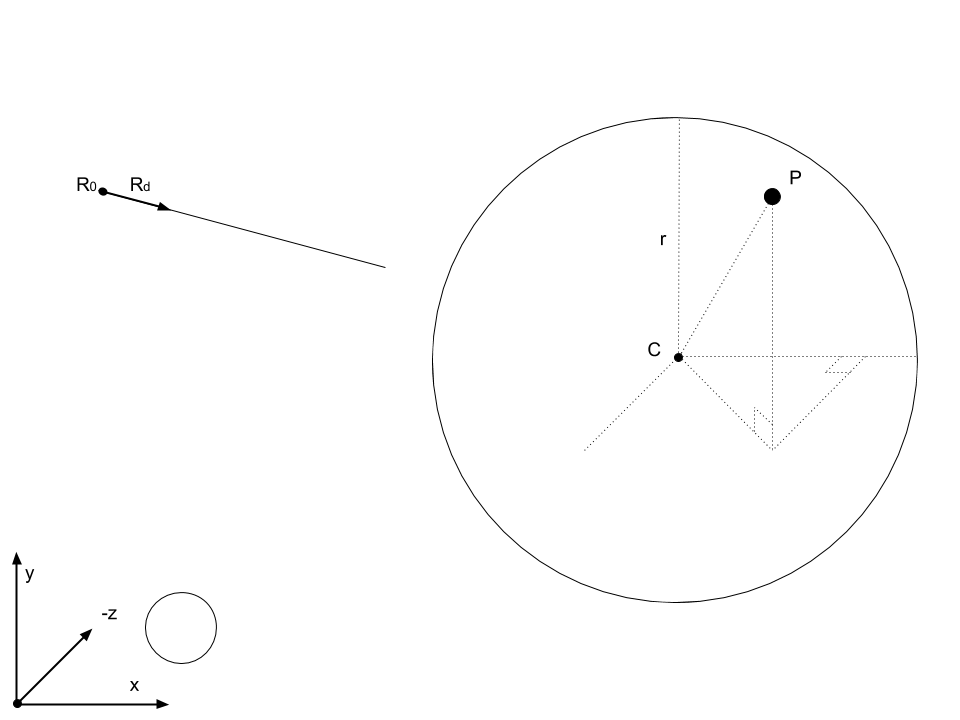
\includegraphics[width=\linewidth]{Figures/ray-sphere-intersection.png}
\decoRule
\caption[ray-sphere-intersection]{Ray-Sphere intersection}
\end{figure}

A point \emph{P} on the surface of sphere should match the equation:

\begin{equation}\label{equ:sphere-surface}
(x_p - x_c)^2 + (y_p - y_c)^2 + (z_p - z_c)^2 = r^2
\end{equation}

If the ray intersects with the sphere at any position\emph{P} must match the equation \ref{equ:ray-t} and \ref{equ:sphere-surface}. Therefor the solution of \emph{t} in the cointegrate equation implies whether or not the ray will intersect with the sphere:

\[
\begin{aligned}
(x_{R_0} + x_{R_d} \cdot t - x_c)^2 &+ (y_{R_0} + y_{R_d} \cdot t - y_c)^2 + (z_{R_0} + z_{R_d} \cdot t - z_c)^2 = r^2 \\
&\vdots \\
x_{R_d}^2\,t^2 &+ (2\,x_{R_d}\,(x_{R_0} - x_c))\,t + (x_{R_0}^2 - 2\,x_{R_0}\,x_c + x_c^2) \\
+\;y_{R_d}^2\,t^2 &+ (2\,y_{R_d}\,(y_{R_0} - y_c))\,t + (y_{R_0}^2 - 2\,y_{R_0}\,y_c + y_c^2) \\
+\;z_{R_d}^2\,t^2 &+ (2\,z_{R_d}\,(z_{R_0} - z_c))\,t + (z_{R_0}^2 - 2\,z_{R_0}\,z_c + z_c^2) = r^2
\end{aligned}
\]

It can be seen as a quadratic formula:

\begin{equation}\label{equ:sphere-surface-quadratic-formula}
a\,t^2 + b\,t + c = 0
\end{equation}

At this point, we are able to solved the \emph{t}:

\[
t =
\begin{cases}
\frac{-b \pm \sqrt{b^2 - 4\,a\,c}}{2\,a} & \text{if }\;b^2 - 4\,a\,c > 0 \\
\frac{-b}{2\,a} & \text{if }\; b^2 - 4\,a\,c = 0 \\
\varnothing & \text{if }\; b^2 - 4\,a\,c < 0
\end{cases}
\]

Then, I take a further step to get rid of formula complexity.

$\because$ Equation \ref{equ:sphere-surface},\,\ref{equ:sphere-surface-quadratic-formula}
\[
\left\{
\begin{array}{lr}
a = x_{R_d}^2 + y_{R_d}^2 + z_{R_d}^2 \\
b = 2\,(x_{R_d}\,(x_{R_0} - x_c) + y_{R_d}\,(y_{R_0} - y_c) + z_{R_d}\,(z_{R_0} - z_c)) \\
c = (x_{R_0} - x_c)^2 + (y_{R_0} - y_c)^2 + (z_{R_0} - z_c)^2 - r^2
\end{array}
\right.
\]

$\And$
\[
\begin{array}{lr}
\begin{aligned}
\norm{\overrightarrow{R_d}} &= \sqrt{x_{R_d}^2 + y_{R_d}^2 + z_{R_d}^2} = 1 \\
\overrightarrow{V_{c\_R_0}} &= \overrightarrow{R_0} - \overrightarrow{C} = \overrightarrow{(x_{R_0} - x_c,\enspace y_{R_0} - y_c,\enspace z_{R_0} - z_c)}
\end{aligned}
\end{array}
\]

$\therefore$
\[
\left\{
\begin{array}{lr}
a =1 \\
b = 2 \cdot \overrightarrow{R_d} \cdot \overrightarrow{V_{c\_R_0}} \\
c = \overrightarrow{V_{c\_R_0}} \cdot \overrightarrow{V_{c\_R_0}} \cdot r^2
\end{array}
\right.
\]

$\because$ The formula for \emph{t} can also be optimized
\[
\left\{
\begin{array}{lr}
\frac{-b \pm \sqrt{b^2 - 4\,a\,c}}{2\,a} = -\alpha \pm \sqrt{\beta} \\
\alpha = 0.5\,b \\
\beta = \alpha^2 - c
\end{array}
\right.
\]

$\therefore$ The final solution for \emph{t}
\[
t =
\begin{cases}
 -\alpha \pm \sqrt{\beta} & \text{if }\;\beta > 0 \\
-\alpha & \text{if }\;\beta = 0 \\
\varnothing & \text{if }\;\beta < 0
\end{cases}
\]

And the collision position for each \emph{t} is:

\[
\overrightarrow{P} = \overrightarrow{R_0} + \overrightarrow{R_d} \cdot t
\]

%****************************************************************
\subsection{Ray-Plane}
\parencite{stackoverflow.ray-plane.2014} \\

\begin{figure}[H]\label{fig:ray-plane}
\centering
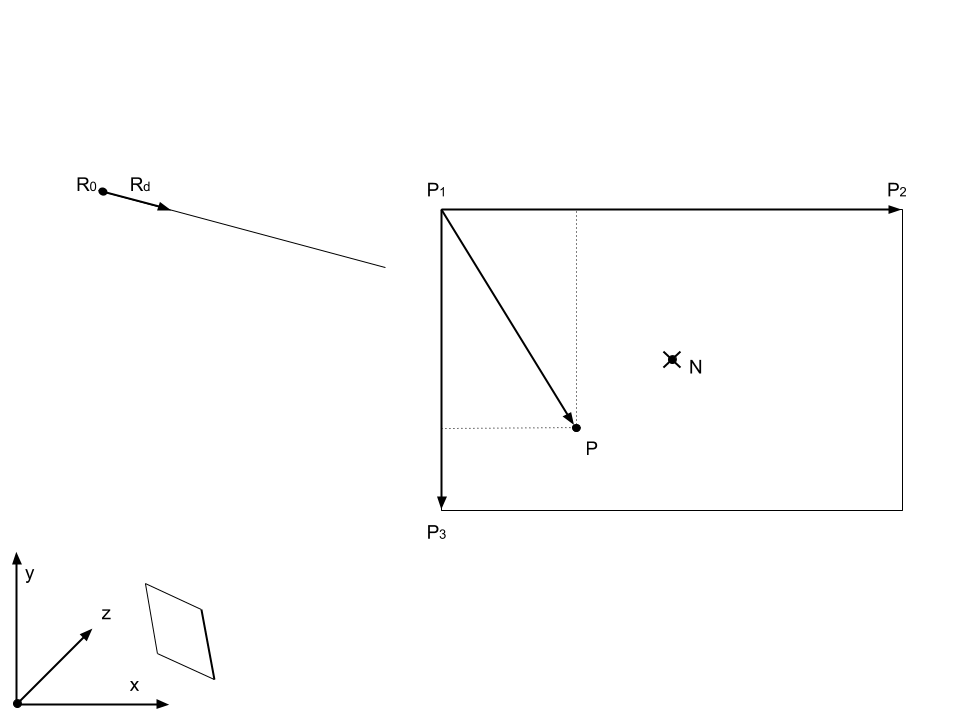
\includegraphics[width=\linewidth]{Figures/ray-plane-intersection.png}
\decoRule
\caption[ray-plane-intersection]{Ray-Plane intersection}
\end{figure}

If a point \emph{P} on the plane and also belongs to the ray, we have quadric equation:

\begin{equation}\label{equ:ray-plane-intersection}
\left\{
\begin{array}{lr}
(\overrightarrow{P} - \overrightarrow{P_1}) \cdot \overrightarrow{N} = 0 \\
\overrightarrow{P} = \overrightarrow{R_0} + \overrightarrow{R_d} \cdot t
\end{array}
\right.
\end{equation}

Solution for the \emph{t} is:

\[
t =
\begin{cases}
\frac{-\overrightarrow{N} \cdot (\overrightarrow{R_0} - \overrightarrow{P_1})}{\overrightarrow{N} \cdot \overrightarrow{R_d}} & \text{if }\;\overrightarrow{N} \cdot \overrightarrow{R_d} \nsim 0 \\
\varnothing & \text{if }\;\overrightarrow{N} \cdot \overrightarrow{R_d} \sim 0
\end{cases}
\]

At last, we have to verify if the collision is inside of the quadrangle by putting \emph{t} back to \ref{equ:ray-plane-intersection}, and the \emph{t} is valid only if:

\[
\begin{array}{lr}
\mu = \sqrt{(\overrightarrow{P} - \overrightarrow{P_1}) \cdot (\overrightarrow{P_2} - \overrightarrow{P_1}))} \in [0,\enspace\norm{\overrightarrow{P_2} - \overrightarrow{P_1}}] \\
\nu = \sqrt{(\overrightarrow{P} - \overrightarrow{P_1}) \cdot (\overrightarrow{P_3} - \overrightarrow{P_1}))} \in [0,\enspace\norm{\overrightarrow{P_3} - \overrightarrow{P_1}}] 
\end{array}
\]

%****************************************************************
\subsection{Ray-Box}
\parencite{Williams.ray-box.2005} \\
\parencite{Tavian.ray-box-2d.2011} \\
\parencite{scratchapixel.ray-plane-3d} \\

There is a octree implementation in the VR 3D world that separate the 3D world to invisible 3D boxes that each box contains a certain number of other models. It is to avoid unnecessary ray-object collision detection. In this section, I am going to first explain Ray-Box-2D collision detection, then derive out Ray-Box-3D intersection.

%****************************************************************
\subsubsection{Ray-Box-2D}

\begin{figure}[H]\label{fig:ray-box-2d}
\centering
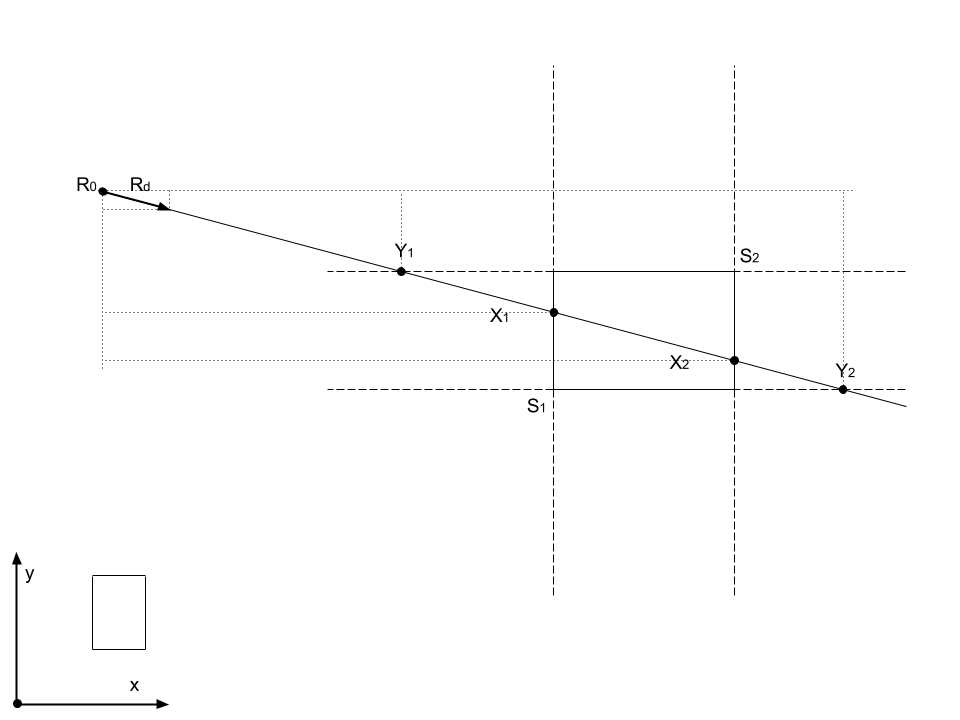
\includegraphics[width=\linewidth]{Figures/ray-box-2d-intersection.png}
\decoRule
\caption[ray-box-2d-intersection]{Ray-Box-2D intersection}
\end{figure}

$\because$ Known $R_0$,\enspace$R_d$,\enspace$P_1$,\enspace$P_2$
\begin{multicols}{2}
\noindent
\[
X_1 =
\begin{cases}
x_{P_1} - x_{R_0} & \text{if }\;x_{R_d} > 0 \\
x_{P_2} - x_{R_0} & \text{if }\;x_{R_d} < 0
\end{cases}
\]
\[
X_2 =
\begin{cases}
x_{P_2} - x_{R_0} & \text{if }\;x_{R_d} > 0 \\
x_{P_1} - x_{R_0} & \text{if }\;x_{R_d} < 0
\end{cases}
\]
\[
\begin{array}{lr}
t_{X_1} = \frac{X_1}{x_{R_d}} \\
t_{X_2} = \frac{X_2}{x_{R_d}}
\end{array}
\]
\columnbreak
\[
Y_1 =
\begin{cases}
y_{P_1} - y_{R_0} & \text{if }\;y_{R_d} > 0 \\
y_{P_2} - y_{R_0} & \text{if }\;y_{R_d} < 0
\end{cases}
\]
\[
Y_2 =
\begin{cases}
y_{P_2} - y_{R_0} & \text{if }\;y_{R_d} > 0 \\
y_{P_1} - y_{R_0} & \text{if }\;y_{R_d} < 0
\end{cases}
\]
\[
\begin{array}{lr}
t_{Y_1} = \frac{Y_1}{y_{R_d}} \\
t_{Y_2} = \frac{Y_2}{y_{R_d}}
\end{array}
\]
\end{multicols}

$\And$ When collision happens,  we have formula
\[
\left\{
\begin{array}{lr}
\begin{aligned}
t_{X_1} &< t_{X_2} \\
t_{Y_1} &< t_{Y_2}
\end{aligned}
\end{array}
\right.
\]

$\therefore$ Which is
\begin{equation}\label{equ:ray-box-2d-intersection}
max(t_{X_1},\enspace t_{Y_1}) < min(t_{X_2},\enspace t_{Y_2})
\end{equation}

%****************************************************************
\subsubsection{Ray-Box-3D}

\begin{figure}[H]\label{fig:ray-box-3d}
\centering
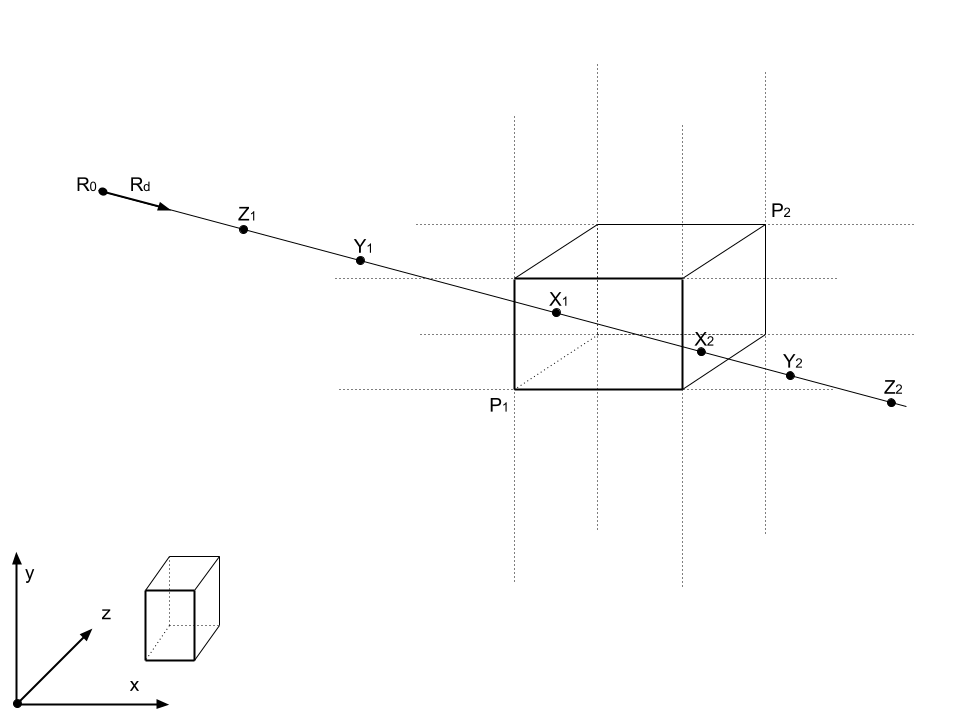
\includegraphics[width=\linewidth]{Figures/ray-box-3d-intersection.png}
\decoRule
\caption[ray-box-3d-intersection]{Ray-Box-3D intersection}
\end{figure}

$\because$ Known $R_0$,\enspace$R_d$,\enspace$P_1$,\enspace$P_2$
\begin{multicols}{2}
\noindent
\[
X_1 =
\begin{cases}
x_{P_1} - x_{R_0} & \text{if }\;x_{R_d} > 0 \\
x_{P_2} - x_{R_0} & \text{if }\;x_{R_d} < 0
\end{cases}
\]
\[
X_2 =
\begin{cases}
x_{P_2} - x_{R_0} & \text{if }\;x_{R_d} > 0 \\
x_{P_1} - x_{R_0} & \text{if }\;x_{R_d} < 0
\end{cases}
\]
\[
\begin{array}{lr}
t_{X_1} = \frac{X_1}{x_{R_d}} \\
t_{X_2} = \frac{X_2}{x_{R_d}}
\end{array}
\]
\columnbreak
\[
Y_1 =
\begin{cases}
y_{P_1} - y_{R_0} & \text{if }\;y_{R_d} > 0 \\
y_{P_2} - y_{R_0} & \text{if }\;y_{R_d} < 0
\end{cases}
\]
\[
Y_2 =
\begin{cases}
y_{P_2} - y_{R_0} & \text{if }\;y_{R_d} > 0 \\
y_{P_1} - y_{R_0} & \text{if }\;y_{R_d} < 0
\end{cases}
\]
\[
\begin{array}{lr}
t_{Y_1} = \frac{Y_1}{y_{R_d}} \\
t_{Y_2} = \frac{Y_2}{y_{R_d}}
\end{array}
\]
\end{multicols}
\begin{multicols}{2}
\noindent
\[
Z_1 =
\begin{cases}
z_{P_1} - z_{R_0} & \text{if }\;z_{R_d} > 0 \\
z_{P_2} - z_{R_0} & \text{if }\;z_{R_d} < 0
\end{cases}
\]
\[
Z_2 =
\begin{cases}
z_{P_2} - z_{R_0} & \text{if }\;z_{R_d} > 0 \\
z_{P_1} - z_{R_0} & \text{if }\;z_{R_d} < 0
\end{cases}
\]
\[
\begin{array}{lr}
t_{Z_1} = \frac{Z_1}{z_{R_d}} \\
t_{Z_2} = \frac{Z_2}{z_{R_d}}
\end{array}
\]
\columnbreak
\[
\]
\end{multicols}

$\And$ When collision happens,  we have formula
\[
\left\{
\begin{array}{lr}
\begin{aligned}
t_{X_1} &< t_{X_2} \\
t_{Y_1} &< t_{Y_2} \\
t_{Z_1} &< t_{Z_2}
\end{aligned}
\end{array}
\right.
\]

$\therefore$ Which is
\begin{equation}\label{equ:ray-box-3d-intersection}
max(t_{X_1},\enspace t_{Y_1},\enspace t_{Z_1}) < min(t_{X_2},\enspace t_{Y_2},\enspace t_{Z_2})
\end{equation}

%****************************************************************
